\documentclass[../deliverable-two.tex]{subfiles}

\begin{document}
\label{ui}

\subsection{Aplikacja kliencka}

Aplikacja kliencka posiada interfejs użytkownika pozwalający na zalogowanie się oraz nawiązanie połączenia ze zdalną sesją. Użytkownikowi wyświetlany jest czynność, która aktualnie się odbywa, oraz w każdym momencie może zakończyć sesję.\\\\

\begin{figure}[H]
  \centering\includegraphics[width=\screenswidth]{client/Login.png}
  \caption{Ekran logowania}
\end{figure}

\begin{figure}[H]
  \centering\includegraphics[width=\screenswidth]{client/Main screen.png}
  \caption{Główny widok zawierający dostępność maszyn}
\end{figure}

Na tym ekranie użytkownik może rozpocząć proces uzyskiwania sesji, przejść do ekranu ustawień lub wylogować się. Jeżeli w systemie nie ma dostępnych maszyn, lub nie uda się uzyskać informacji o ich dostępności, to przycisk połączenia jest niedostępny. Wciśnięcie tego przycisku prowadzi do kolejnego ekranu.

\begin{figure}[H]
  \centering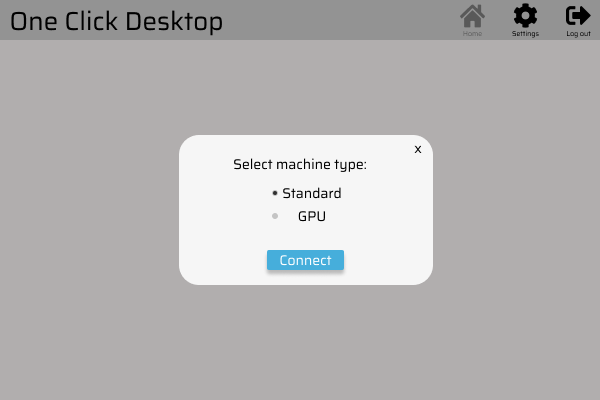
\includegraphics[width=\screenswidth]{client/Connect modal.png}
  \caption{Wybór typu sesji}
\end{figure}

Do wyboru dostępne są jedynie typy sesji, które system określi jako dostępne. Wybranie typu sesji kliknięcie przycisku prowadzi do kolejnego ekranu. Następne ekrany przechodzą automatycznie do kolejnych bez interwencji użytkownika, aż do informacji o nawiązaniu połączenia lub błędu.\\\\

\begin{figure}[H]
  \centering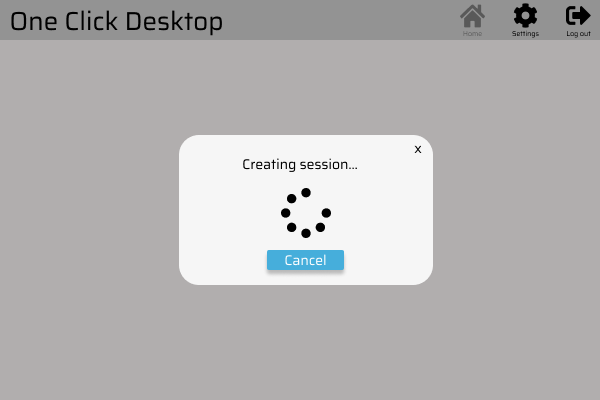
\includegraphics[width=\screenswidth]{client/Creating session.png}
  \caption{Tworzenie sesji}
\end{figure}

\begin{figure}[H]
  \centering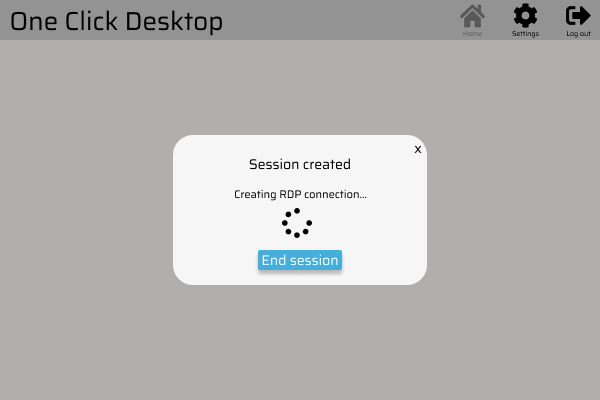
\includegraphics[width=\screenswidth]{client/Connecting modal.png}
  \caption{Nawiązywanie połączenia RDP}
\end{figure}

\begin{figure}[H]
  \centering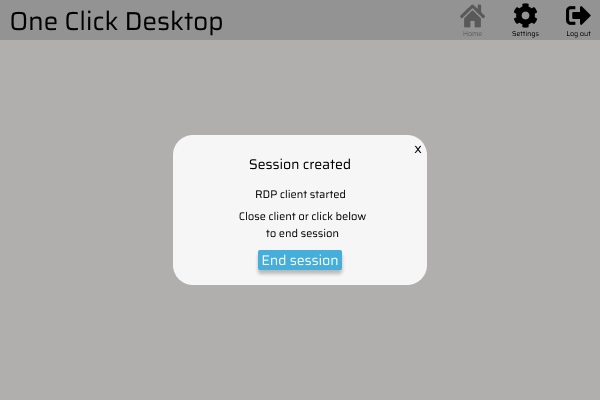
\includegraphics[width=\screenswidth]{client/RDP connecting.png}
  \caption{Połączenie nawiązane}
\end{figure}

\begin{figure}[H]
  \centering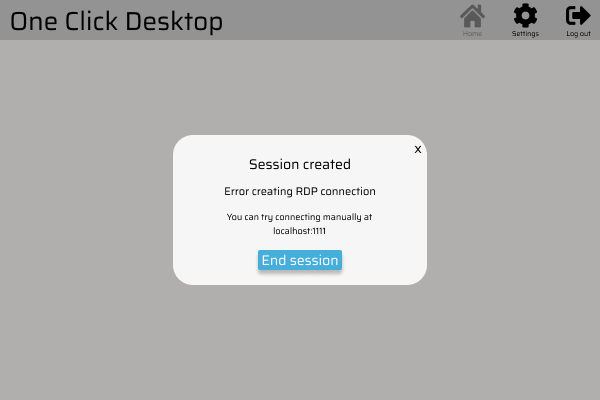
\includegraphics[width=\screenswidth]{client/RDP cannot connect.png}
  \caption{Błąd przy nawiązywaniu połączenia}
\end{figure}

\begin{figure}[H]
  \centering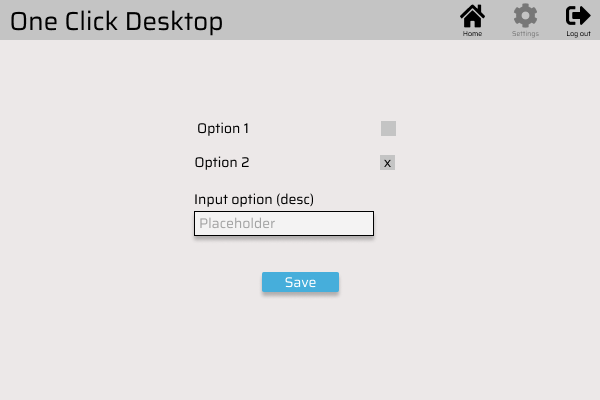
\includegraphics[width=\screenswidth]{client/Settings.png}
  \caption{Ustawienia}
\end{figure}

\begin{figure}[H]
  \centering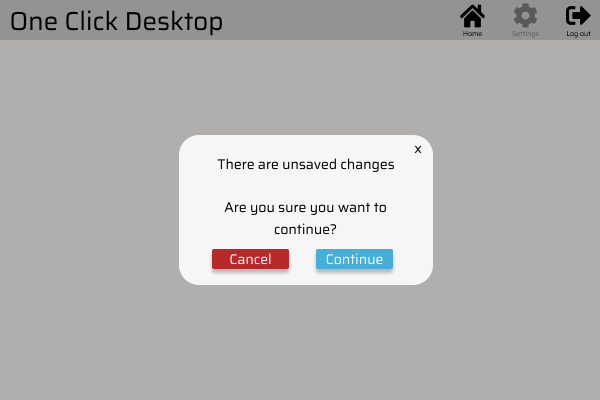
\includegraphics[width=\screenswidth]{client/Setting not saved changes.png}
  \caption{Powiadomienie przy wyjściu z ekranu ustawień z niezapisanymi zmianami}
\end{figure}

\pagebreak

\subsection{Panel administratora}

Panel administratora posiada skromny interfejs umożliwiający zalogowanie się oraz podgląd zużycia zasobów.

\begin{figure}[H]
  \centering\includegraphics[width=\screenswidth]{admin/Login.png}
  \caption{Ekran logowania}
\end{figure}

\begin{figure}[H]
  \centering\includegraphics[width=\screenswidth]{admin/Main screen.png}
  \caption{Widok zużycia zasobów}
\end{figure}

Na tym widoku możemy zobaczyć zużycie zasobów globalne oraz dla każdego z serwerów wirtualizacji. Dodatkowo dla serwera wyświetlona jest również ilość działających i możliwych do uruchomienia maszyn każdego z typów.

\end{document}